\documentclass[11pt]{aghdpl}
\graphicspath{ {img/} }
\usepackage{svg}
% \documentclass[en,11pt]{aghdpl}  % praca w języku angielskim

% Lista wszystkich języków stanowiących języki pozycji bibliograficznych użytych w pracy.
% (Zgodnie z zasadami tworzenia bibliografii każda pozycja powinna zostać utworzona zgodnie z zasadami języka, w którym dana publikacja została napisana.)
\usepackage[english,polish]{babel}

% Użyj polskiego łamania wyrazów (zamiast domyślnego angielskiego).
\usepackage{polski}

\usepackage[utf8]{inputenc}

% dodatkowe pakiety

\usepackage{mathtools}
\usepackage{amsfonts}
\usepackage{amsmath}
\usepackage{amsthm}

% --- < bibliografia > ---

\usepackage[
style=numeric,
sorting=none,
%
% Zastosuj styl wpisu bibliograficznego właściwy językowi publikacji.
language=autobib,
autolang=other,
% Zapisuj datę dostępu do strony WWW w formacie RRRR-MM-DD.
urldate=edtf,
% Nie dodawaj numerów stron, na których występuje cytowanie.
backref=false,
% Podawaj ISBN.
isbn=true,
% Nie podawaj URL-i, o ile nie jest to konieczne.
url=false,
%
% Ustawienia związane z polskimi normami dla bibliografii.
maxbibnames=3,
% Jeżeli używamy BibTeXa:
backend=bibtex
]{biblatex}

\usepackage{csquotes}
% Ponieważ `csquotes` nie posiada polskiego stylu, można skorzystać z mocno zbliżonego stylu chorwackiego.
\DeclareQuoteAlias{croatian}{polish}

\addbibresource{bibliografia.bib}

% Nie wyświetlaj wybranych pól.
%\AtEveryBibitem{\clearfield{note}}


% ------------------------
% --- < listingi > ---

% Użyj czcionki kroju Courier.
\usepackage{courier}

\usepackage{listings}
\lstloadlanguages{TeX}

\lstset{
	literate={ą}{{\k{a}}}1
           {ć}{{\'c}}1
           {ę}{{\k{e}}}1
           {ó}{{\'o}}1
           {ń}{{\'n}}1
           {ł}{{\l{}}}1
           {ś}{{\'s}}1
           {ź}{{\'z}}1
           {ż}{{\.z}}1
           {Ą}{{\k{A}}}1
           {Ć}{{\'C}}1
           {Ę}{{\k{E}}}1
           {Ó}{{\'O}}1
           {Ń}{{\'N}}1
           {Ł}{{\L{}}}1
           {Ś}{{\'S}}1
           {Ź}{{\'Z}}1
           {Ż}{{\.Z}}1,
	basicstyle=\footnotesize\ttfamily,
}

% ------------------------

\AtBeginDocument{
	\renewcommand{\tablename}{Tabela}
	\renewcommand{\figurename}{Rys.}
}

% ------------------------
% --- < tabele > ---

\usepackage{array}
\usepackage{tabularx}
\usepackage{multirow}
\usepackage{booktabs}
\usepackage{makecell}
\usepackage[flushleft]{threeparttable}

% defines the X column to use m (\parbox[c]) instead of p (`parbox[t]`)
\newcolumntype{C}[1]{>{\hsize=#1\hsize\centering\arraybackslash}X}


%---------------------------------------------------------------------------

\author{Michał Gandor}
\shortauthor{M. Gandor}

%\titlePL{Przygotowanie bardzo długiej i pasjonującej pracy dyplomowej w~systemie~\LaTeX}
%\titleEN{Preparation of a very long and fascinating bachelor or master thesis in \LaTeX}

\titlePL{Symulacja dynamiki pieszych z wykorzystaniem modelu Social Force.}
\titleEN{Simulation of pedestrian dynamics using Social Force Model.  }

\shorttitlePL{Symulacja dynamiki pieszych z wykorzystaniem modelu Social Force.}
\shorttitleEN{Simulation of pedestrian dynamics using Social Force Model.  }

\thesistype{Praca dyplomowa inżynierska}
%\thesistype{Master of Science Thesis}

\supervisor{dr hab. inż. Jarosław Wąs}
%\supervisor{Marcin Szpyrka PhD, DSc}

\degreeprogramme{Informatyka}
%\degreeprogramme{Computer Science}

\date{2017}

\department{Katedra Informatyki Stosowanej}
%\department{Department of Applied Computer Science}

\faculty{Wydział Elektrotechniki, Automatyki,\protect\\[-1mm] Informatyki i Inżynierii Biomedycznej}
%\faculty{Faculty of Electrical Engineering, Automatics, Computer Science and Biomedical Engineering}

\acknowledgements{Serdecznie dziękuję \dots tu ciąg dalszych podziękowań np. dla promotora, żony, sąsiada itp.}


\setlength{\cftsecnumwidth}{10mm}

%---------------------------------------------------------------------------
\setcounter{secnumdepth}{4}
\brokenpenalty=10000\relax

\begin{document}

\titlepages

% Ponowne zdefiniowanie stylu `plain`, aby usunąć numer strony z pierwszej strony spisu treści i poszczególnych rozdziałów.
\fancypagestyle{plain}
{
	% Usuń nagłówek i stopkę
	\fancyhf{}
	% Usuń linie.
	\renewcommand{\headrulewidth}{0pt}
	\renewcommand{\footrulewidth}{0pt}
}

\setcounter{tocdepth}{2}
\tableofcontents
\clearpage

\chapter{Wprowadzenie}
\label{cha:wprowadzenie}

Zachowanie tłumu badane jest od przeszło trzech dekad. Na samym początku badania były traktowane w ramach ciekawostki. Wraz z nowatorskimi pracami Helbinga .... . W ostatnich latach zagadnienie to zyskuje coraz większe znaczenie. Jesteśmy obecnie świadkami rozrostu miast, budowy kompleksów sportowych czy galerii handlowych. Wszystkie te miejsca są nieodłącznie związane z tłumami przewijających się przez nie osób. W związku z rosnącą gęstością zaludnienia oraz wzrostem zagoreń takich jak terroryzm [jakis przypis] tworzenie symulacji ewakuacji nabrało większego znaczenia. Dzięki zasymulowaniu zachowania tłumu możenmy łatwiej utworzyć schematy opuszczenia bynków podczaz zagorżenia minimaliusjąc szkody oraz ofiary. Symulacje pozwalają także na lepsze rozładowanie ruchu drogowego w miastach o roznącej ilości zaludnienia.

Symulacje mogą mieć wielorakie zastosowanie, począwszy od ewakucaji ludności poprzez zachowania w centrach handlowych kończąc na ruchu drogowym. Na przejściach dla pieszych w Japonii ginie 30\% osób uczestniczących w wypadkach drogowych \cite{AMSFMfPBSaSC}, a w Niemczech odsetek ten wynosi 15\% \ [German instigute for econeomic research 2010]. Zgodnie z danymi organizacjie Fire Administration w Stanach Zjednoczonych \cite{Asfemwle} w roku 2007 3430 osób zmarło w pożarach oraz blisko 18 tysięcy zostało ranych.

%---------------------------------------------------------------------------

\section{Cele pracy}
\label{sec:celePracy}

Celem poniższej pracy jest zapoznanie studentów z systemem \LaTeX~w zakresie umożliwiającym im samodzielne, profesjonalne złożenie pracy dyplomowej w systemie \LaTeX.

%---------------------------------------------------------------------------

\section{Zawartość pracy}
\label{sec:zawartoscPracy}

W rodziale~\ref{cha:pierwszyDokument} przedstawiono podstawowe informacje dotyczące struktury dokumentów w \LaTeX u. Alvis~\cite{Alvis2011} jest językiem 



















\chapter{Wykaz ważniejszych oznaczeń}
\label{sec:wykazOznaczen}

SFM - Social Force Model
A* - algorytm A Star
POI - points of intrests
[do dopisania]

















\chapter{Wprowadzenie teoretyczne}
\label{cha:wprowadzenieTeoretyczne}

Dziedziny nauki badające ruch pieszych to nie tylko informatyka. Na powstanie modeli miały także wpływ prace uczonych z takich dziedzin jak psychologia, socjologia czy architektura. Problem zachowania tłumu jest skomplikowany i dopiero połączenie tych wszystkich dziedzin dało początek realnemu odzwierciedleniu na ekranie komputera. \\
Z pozoru zachowanie pieszych może wydawać się chaotyczne oraz trudne do przewidzenia. Bazując jednak na badaniach i obserwacjach takie zachowania mają miejsce tylko w skrajnych przypadkach. W codziennym życiu okazuje się, że model do opisu zachowania tłumu może być w dość prosty sposób opisany, głównie dzięki prawdopodobieństwom jakie mogą zostać nakreślone w dużych populacjach ludzi. Człowiek ma tendencję do podejmowania decyzji na bazie posiadanej już wcześniej, wypracowanej wiedzy na temat otaczającego go środowiska. Oznacza to, że reakcje na innych pieszych oraz przeszkody mogą być w łatwy sposób przewidziane. Analogią do takiego zachowania mogą być przykładowo reakcje profesjonalnego kierowcy wyścigowego, który reaguje na sytuacje drogowe niemal automatycznie.

Oczywiście nie jest to prawdą w każdej sytuacji. Przykładowo dzieci oraz turyści wykazują inny sposób poruszania się za względu na to, że zazwyczaj znajdują się w nowym miejscu i nie mają wypracowanej strategii poruszania się. Jednakże dla potrzeb symulacji nie potrzeba dokładnych informacji o każdym z pieszych. W zupełności wystarcza statystyczna wartość konkretnych zachowań

W tym rozdziale zostają przedstawione podstawowe dostępne obecnie modele. Każdy z modeli ma swoje zalety oraz wady, wpływają na to cechy takie jak złożoność obliczeniowa, złożoność implementacji oraz oczywiście cechy otrzymanych rezultatów.

\section{Klasyfikacja modeli symulacji ruchu pieszych}
\label{sec:klasyfikacja}

\subsection{Modele mikroskopowe oraz makrospokope}

Modele makroskopowe pokazują w głównej mierze dynamikę gęstości oraz prędkości całego tłumu. W tym celu używane są istniejące już modele fizyczne takie jak dynamika płynów, które zostają odpowiednio dostosowane do potrzeb symulacji. Przykładem może być hydrodynamiczny model Paulusa opierający się na równaniach przepływu \cite{ArchitekturaModelowania}. Modele te nie biorą pod uwagę indywidualnych zachowań jednostki.\\

Podejście makrospokowe ze względu na odzwierciedlanie całej populacji sprawdza się w praktyce tylko w wąskim wachlarzu zastosowań.
 
Jako zaletę podejścia makroskopowego możemy z pewnością wskazać mniejszą ilość obliczeń potrzebną do uzyskania porządanego efektu.

Modele mikrospokowe, w przeciwieństwie do wspomnianych wyżej modeli makroskopowych, biorą one pod uwagę zachowanie konkretnej jednostki. Badane są interakcje pomiędzy pieszymi oraz ich iteracje z przeszkodami oraz otaczającą rzeczywistością. Modele te pozwalają na uzyskanie efekty bardziej odpowiadającego realnemu zachowaniu tłumu. Jednakże wraz ze wzrostem odwzorowania detali wzrasta również złożoność systemu oraz zwiększa się złożoność obliczeń co skutkuje toeretycznie gorszą wydajnością, jednak przy dostępnej obecnie mocy obliczeniowej nawet standardowych komputerów nie gra to aż takiej roli.

\subsection{Modele ciągłe i dyskretne}

W modelach mikroskopowych możemy wyodrębinić dwie podgrupy: modele ciągłe oraz dyskretne. Modele dyskretne cechują się zmianą paramatrów stanu w konkretnych interwałąch czasowych, przyjmują okręślone wartości dla określonych argumantów i tylko dla nich. W modelach ciągłych stan ulega zmienie przez cały czas działania, może przyjmować dowonlą wartość z całego przedziału. Modele ciągłe reprezentują oczywiście dane w sposób bardziej realistyczny, jednakże zwiększają czas obliczeń \\

Jednym z przykładów na model dyskretny może być automat komórkowy. Uniwersalność automatów komórkowych \textit{Cellular Automata} spowodowała, iż znajdują zastosowanie także w dziedzinie symulacji ruchu pieszych. Automat komórkowy jest modelem matematycznym, który specyfikuje siatka komórek, zbiór stanów jakie mogą one przyjmować, oraz reguły określające stan komórki w chwili $t + 1$. Stan danej komórki zależny jest od stanu komórek z nią sąsiadujących w chwili $t$. \\

Dla stworzenia modeli mikroskopowych używano z początku niehomogenicznych automatów komórkowych. Wraz z rozwojem symulacji na automatach komórkowych można było dostrzec duże zmiany bazowym modelu. Powstające symulacje zaczęły zostać klasyfikowane jako \textbf{sytemy agentowe}.

Niestety jednorodność tej metody uniemożliwia modelowanie bardziej skomplikowanych procesów\cite{FormalizacjaAutomatów}.

%---------------------------------------------------------------------------



















\chapter{Opis modelu Social Force}
\label{cha:OpisSocialForce}

Model Social Force \cite{SforceModelForPedDyn}, bezsprzecznie najważniejszy z obecnie dostępnych, jest mikrospokowym modelem ciągłym. Zakłada on, że piesi w ruchu mogą zostać w prosty sposób opisani za pomocą sił. Siły te pochodzą nie tylko z oddziaływań konkretnego pieszego na otoczenie, ale także z otoczenia na danego pieszego. Wartość, zwrot oraz kierunek siły finalnej jest składową wszystkich sił działających na danego pieszego. Piesi w modelu reprezentowani są za pomocą cząstek, które dążą do celu w konkretnych kierunkach oraz są pod działaniem wspomnianych sił. Dotychczasowe symulacje komputerowe pokazują, że Model Social Force, pomimo swojej prostoty bardzo realistycznie oddaje rzeczywiste zachowanie tłumu.

\begin{figure}
\centering
\includegraphics[width=0.5\textwidth]{process.eps}
\caption{Schemat podejmowania decyzji przez pieszego, opracowanie własne na bazie \cite{GuideCrowdDynViaModifiedSocialForceModel}}
\end{figure}

Nie bez znaczenia jest także łatwość uzyskania parametrów oraz wartości potrzebnych do symulacji. Wartości takie jak predkość $\vec{v_{\alpha}}$ czy położenie $\vec{r_{\alpha}}$ danego pieszego $\alpha$ są łatwe do obliczenia, ale także do skalibrowania z danami empirycznymi.

Pierwsze symulacje korzystające z modelu SF były skupione głównie na ewakuacjach budynków. W tego typu sytuacjach celem pieszego jest dojście do wyjścia w możliwie najkrótszym czasie. Obecnie istnieje mnogość wariantów modelu, które pozwalają na zamodelowanie większej ilości zachowań. Obecne modyfikacje przewidują przykładowo unikanie "spychania" innych uczestników ruchu poprzez pieszych poruszających się z większą prędkością \cite{6}.

Istnieje bardzo wiele różnych modyfikacji modelu Social Forca. Wykorzystany w pracy model \cite{GuideCrowdDynViaModifiedSocialForceModel} bazuje na oryginalnym modelu Helbinga \cite{SforceModelForPedDyn} zakłada, że na pieszego działają trzy siły. Desired force $\vec{f_{i}^{0}}$, siła interakcji pomiędzy pieszymi $i$ oraz $j$, $\vec{f_{ij}}$ oraz siła interakcji pomiędzy pieszym $i$, a przeszkodami, $\vec{f_{iw}}$

Siła działająca na każdego z pieszych definiuje się jako:

\begin{equation}
m_{i} \frac{d\vec{v_{i}}(t)}{dt} = \vec{f_{i}^{0}} + \sum_{j(\neq i)} \vec{f_{ij}} + \sum _{w} \vec{f_{iw}}
\end{equation}

gdzie
\begin{eqwhere}[2cm]
	\item[$m_{i}$] masa pieszego $i$
	\item[$\vec{v}_{i}(t)$] aktualna prędkość
\end{eqwhere}

\section{Desired force}
\label{sec:desiredForce}

Bazując na obserwacjach można wywnioskować, że piesi wykazują niechęć do zmiany prędkości oraz kierunku swojej drogi. Zazwyczaj wybierana jest droga, którą można podążać prosto przez jak najdłuższy okres czasu, nawet jeśli drogi alternatywne są takiej samej długości, a droga wybrana przez pieszego jest mocno zatłoczona. Kierunek ruchu obliczany jest na podstawie wzoru:

\begin{equation}
\vec{e}_{\alpha}(t) = \frac{\vec{r}_{\alpha}^{k} - \vec{r}_{\alpha}(t)}{\parallel \vec{r}_{\alpha}^{k} - \vec{r}_{\alpha}(t) \parallel}
\end{equation}

gdzie
\begin{eqwhere}[2cm]
	\item[$e_{\alpha}(t)$] aktualna pozycja pieszego $\alpha$ w czasie $t$
	\item[$\vec{r}_{\alpha}^{k}$] najbliższy punkt na ścieżce do celu
\end{eqwhere}

\begin{figure}
\centering
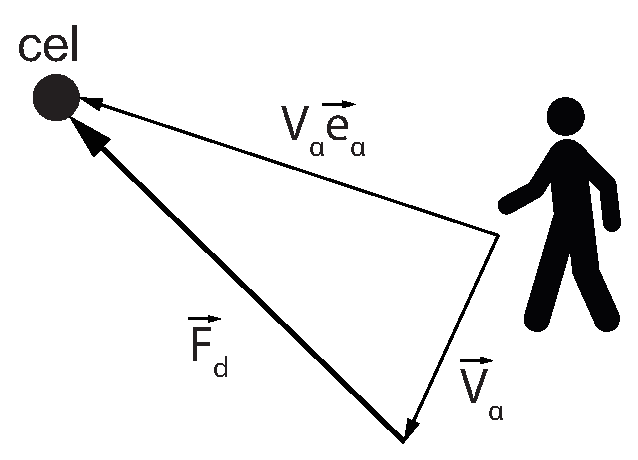
\includegraphics[width=0.5\textwidth]{desiredforce2.eps}
\caption{Schemat siły \textit{desired force} , opracowanie własne na bazie \cite{AMSFMfPBSaSC}}
\end{figure}

\begin{figure}
\centering
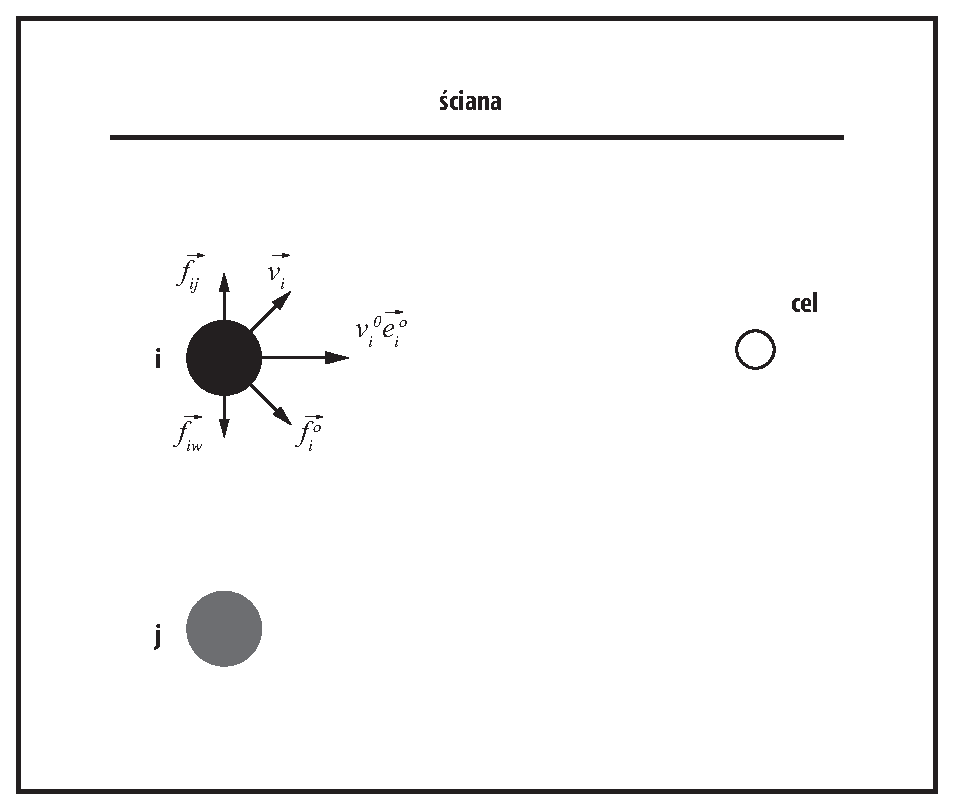
\includegraphics[width=0.5\textwidth]{desiredforce.eps}
\caption{Diagram modelu Social Force, opracowanie własne na bazie \cite{GuideCrowdDynViaModifiedSocialForceModel}}
\end{figure}

W przypadku kiedy ruch pieszego odbywa się bez przeszkód porusza się on w kierunku pozycji celu, z preferowaną przez siebie prędkością, $\vec{v_{i}^{0}}$. Z powodu działania na pieszego sił~z otoczenia, obserwuje się dążenie pieszego do osiągnięcia preferowanej przez siebie prędkości w czasie relaksacji $\tau$.

\begin{equation}
\vec{f}_{i}^{0} = m_{i} \frac{v_{i}^{0}(t) \vec{e_{i}^{0}} - \vec{v_{i}}(t)}{\tau}
\end{equation}

gdzie
\begin{eqwhere}[2cm]
	\item[$\vec{v_{i}^{0}}$] wartość domyślnej prędkości pieszego
	\item[$\vec{e_{i}^{0}}$] kierunek ruchu jaki pieszy chce osiągnąć
	\item[$\tau$] czas relaksacji
\end{eqwhere}
	
Jest to tzw. \textit{desired speed} [wyjaśnić], odzwierciedla ona dążenie danego pieszego $i$ do osiągnięcia preferowanej prędkości.

Domyślna prędkość pieszego przyjmuje zazwyczaj wartość około $1.34 \frac{m}{s^{2}}$ z odchyleniem standardowym $0.26 \frac{m}{s^{2}}$ \cite{HeBuAjTw}

\section{Interakcja pomiędzy pieszymi}
\label{sec:interactionBetweenPedestrians}

Naturalnym jest, że kiedy zbliżamy się do innych uczestników ruchu czujemy się niekomfortowo. Zakłada się, że każdy z pieszych, który jest w konflikcie z innym uczestnikiem ruchu generuje wokół siebie eliptyczne pole siły, które działa na drugiego z pieszych. Aby uniknąć wypadków utrzymują dystans pomiędzy innymi uczestnikami ruchu oraz przeszkodami. Dystans ten zmniejsza się w przypadku kiedy pieszy śpieszy się oraz kiedy wzrasta gęstość tłumu. Gęstość tłumu zwiększa się w szczególności kiedy piesi znajdują się w okolicy miejsc wywierających zainteresowanie oraz w wąskich przejściach. Siła interakcji pomiędzy pieszymi $i$ oraz $j$, $\vec{f_{ij}}$ definiowana jest jako suma dwóch sił, socjologiczno-psychologicznej oraz fizycznej. Piesi mogą także formować grupy, których zachowanie można później sprowadzić do opisu pojedynczego agenta \cite{HeBuAjTw}

\begin{equation}
\vec{f_{ij}} = \vec{f}_{ij}^{s} + \vec{f}_{ij}^{p}
\end{equation}
Pierwsza z nich $\vec{f_{ij}^{s}}$ związana jest z naturalnym ludzkim odruchem utrzymywania dystansu od drugiego człowieka. Przyjmuje ona wartość maksymalną, gdy odległość między dwoma pieszymi $d_{ij}$ maleje, a wartość mniejszą w przypadku oddalania się pieszych.

\begin{equation}
\vec{f_{ij}^{s}} = A_{i} exp[(r_{ij} - d_{ij}) / B_{i}]\vec{n_{ij}}
\end{equation}

gdzie
\begin{eqwhere}[2cm]
	\item[$A_{i}$] Moc siły
	\item[$B_{i}$] Dystans działania siły
	\item[$\vec{n_{ij}}$] wektor jednostkowy o początku w centrum strefy prywatnej pieszego $i$ a końcu w centrum tej strefy pieszego $j$
\end{eqwhere}

Druga z sił $\vec{f_{ij}^{p}}$ wywiera nacisk na pieszych kiedy dystans pomiędzy dwoma pieszymi, $d_{ij}$ jest mniejszy od sumy promieni ich stref prywatnych $r_{ij} = r_{i} + r_{j}$. Siła ta składa się z "body force", $\vec{f} _{ij}^{p_{1}}$ oraz \textit{sliding friction force}, $\vec{f} _{ij}^{p_{2}}$.

\begin{equation}
\vec{f}_{ij}^{p} = kg(r_{ij} - d_{ij}) \vec{n}_{ij} + \kappag (r_{ij} - d_{ij}) \Delta v _{ij}^{t} \vec{t}_{ij}
\end{equation}

gdzie
\begin{eqwhere}[2cm]
	\item[$k$] body compression coefficient
	\item[$\kappa$] Coeficient of sliding friction
	\item[$\vec{n}_{ij}$] wektor jednostkowy o początku w pozycji pieszego $i$ a końcu w pozycji pieszego $j$
	\item[$\Delta v_{ij}^{t} * \vec{t}_{ij}$] zmiana prędkości wzdłuż stycznej do eliptycznego pola strefy prywatnej
\end{eqwhere}

\begin{equation}
g(x) = \lbrace {0, if x < 0, x if x \geq 0.}
\end{equation}

Warto zaznaczyć, że druga z sił przyjmuje pewne wartości nawet w przypadku kiedy dwoje pieszych znajduje się daleko od siebie. Oznacza to, że piesi zawsze starają się utrzymać dystans od siebie nawzajem \cite{relativeVelocity}.


\section{Zalety oraz wady Modelu Social Foce}

Największą z zalet opisywanego modelu jest precyzja odwzorowania zachowań mikroskopowych oddziaływań pomiędzy pieszymi oraz otaczającą ich rzeczywistością. SFM pokazuje także wiele znanych zachowań takich jak:

\begin{itemize}
\item Unikanie kontaktu z przeszkodami oraz innymi uczestnikami ruchu przed dojściem do kolizji,
\item \textit{Szybciej znaczy wolniej}, im szybciej pieszy próbuje się poruszać tym bardziej zatłoczone stają się miejsca takie jak obszary wyjścia z budynków co skutkuje spowolnieniem ruchu,
\item formowanie strug, w korytarzach piesi próbują poruszać się w liniach. Zachowanie to może być zauważone w szczególności kiedy dwie grupy ludzi poruszają się w przeciwnych kierunkach.
\end{itemize}
Wśród wielu zalet modelu możemy wskazać także wady. Pierwszą z nich jest mała wydajność obliczeniowa oraz trudności z odwzorowaniem niektórych sytuacji. Mnogość sił, które są obliczane w przemnożeniu poprzez ilość pieszych powoduje wysoki narzut na ilość obliczeń. W tym miejscu dużą konkurencją stają się automaty komórkowe, które nie wymagają tak skomplikowanych obliczeń dając jednocześnie szerokie spektrum odwzorowania zróżnicowanych zachowań ruchu pieszych.


% itd.
% \appendix
% \begin{titlepage}\centering
\vspace*{\fill}
\LARGE Dodatki
\vspace*{\fill}
\end{titlepage}

\begin{samepage}

\chapter{A. Zbiorcze porównanie testów}
\label{cha:dodatekA}

\begin{figure}
\label{figure:siatka}
\centering
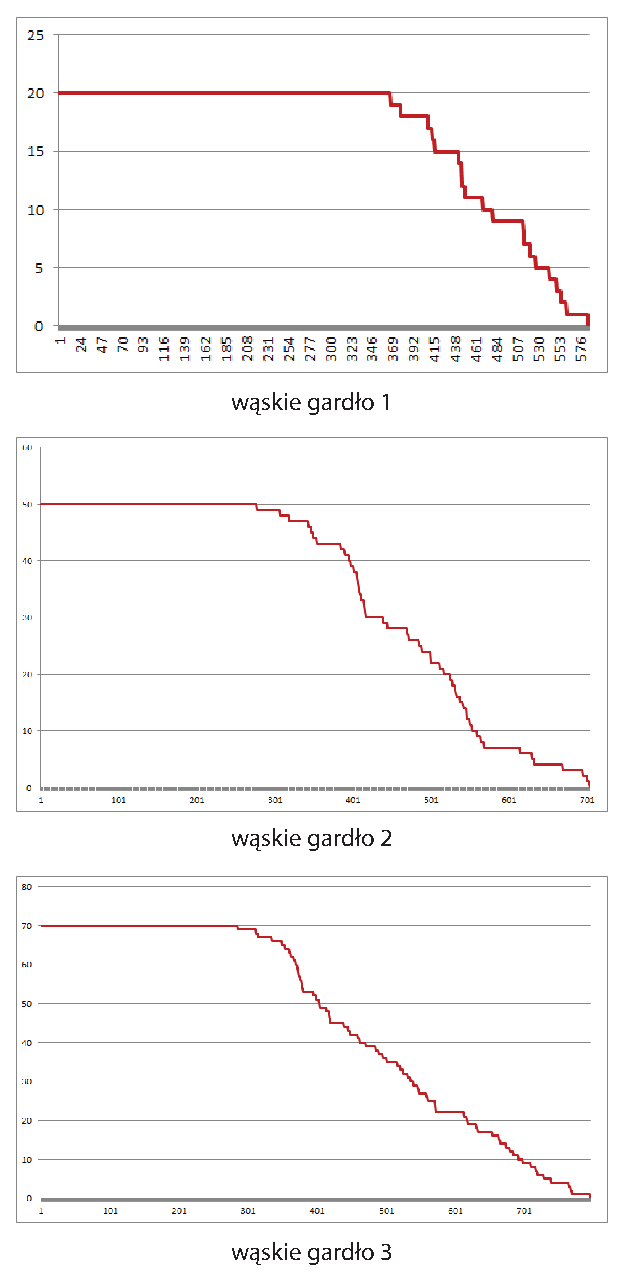
\includegraphics[width=0.4\textwidth]{iloscpieszychwaskie.eps}
\caption{Liczba pieszych w czasie - wąskie gardło}
\end{figure}
\end{samepage}

\begin{figure}
\label{figure:siatka}
\centering
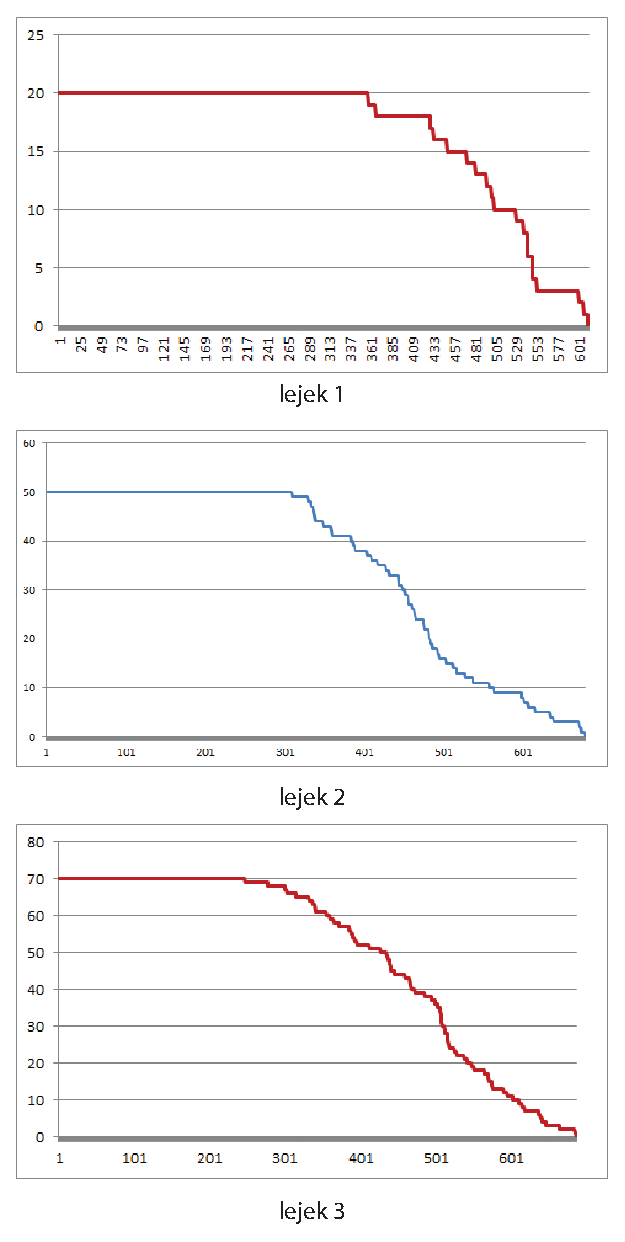
\includegraphics[width=0.5\textwidth]{iloscpieszychlejek.eps}
\caption{Liczba pieszych w czasie - lejek}
\end{figure}

\begin{figure}
\label{figure:siatka}
\centering
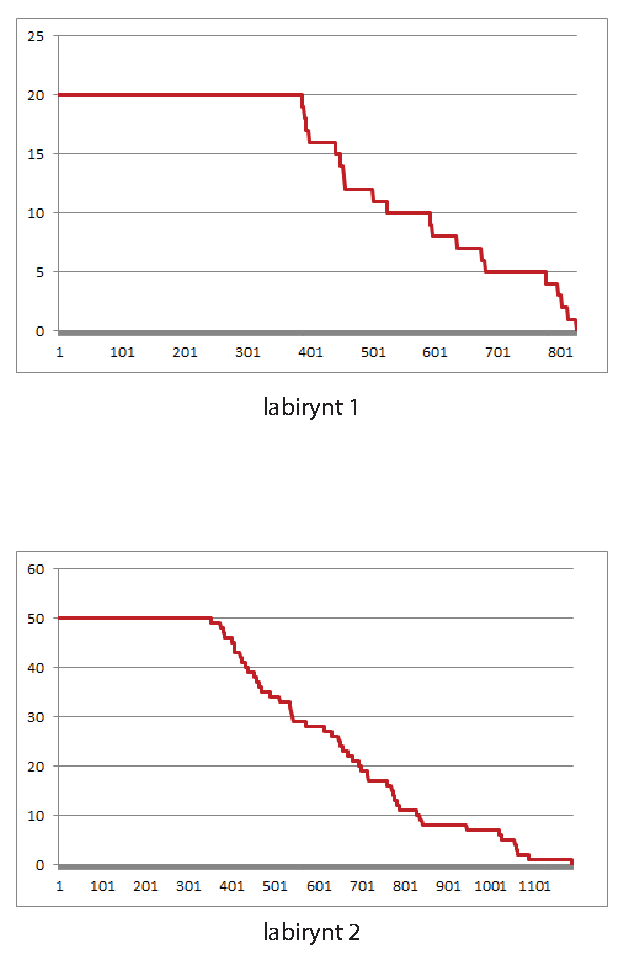
\includegraphics[width=0.5\textwidth]{iloscpieszychlabirynt.eps}
\caption{Liczba pieszych w czasie - labirynt}
\end{figure}

% \include{dodatekB}
% itd.

\printbibliography

\end{document}
